\documentclass[a4paper,german,12pt,smallheadings]{scrartcl}
\usepackage[T1]{fontenc}
\usepackage[utf8]{inputenc}
\usepackage{babel}
\usepackage{geometry}
\usepackage[fleqn]{mathtools} % also includes mathclap
\usepackage[fleqn]{amsmath}
\usepackage{amssymb}
\usepackage{float}
\usepackage{enumerate}
\usepackage{commath} % http://tex.stackexchange.com/questions/14821/whats-the-proper-way-to-typeset-a-differential-operator
\usepackage{cancel}

% Number only referenced equations
\mathtoolsset{showonlyrefs}

%\usepackage{wrapfig}
\usepackage[thinspace,thinqspace,squaren,textstyle]{SIunits}

% New command for color underlining
\usepackage{xcolor}

\newsavebox\MBox
\newcommand\colul[2][red]{{\sbox\MBox{$#2$}%
  \rlap{\usebox\MBox}\color{#1}\rule[-1.2\dp\MBox]{\wd\MBox}{0.5pt}}}

\restylefloat{table}
\geometry{a4paper, top=15mm, left=10mm, right=20mm, bottom=20mm, headsep=10mm, footskip=12mm}
\linespread{1.2}
\setlength\parindent{0pt}
\DeclareMathOperator{\Tr}{Tr}
\DeclareMathOperator{\Var}{Var}
\newcommand*\laplace{\mathop{}\!\mathbin\Delta}
\begin{document}
\allowdisplaybreaks % Seitenumbrüche in Formeln erlauben
\begin{center}
\bfseries % Fettdruck einschalten
\sffamily % Serifenlose Schrift
\vspace{-40pt}
Theoretische Elektrodynamik, Sommersemester 2014, Aufgabenblatt 10

Markus Fenske, Mattis Riediger, Tutor: Clemens Meyer zu Rheda
\vspace{-10pt}
\end{center}

\section*{Aufgabe 1: Magnetisierte Eisenkugel}
\begin{enumerate}[a)]
  \item
Das elektrische Feld der Kugel ist
\begin{equation}
  \vec{E} = \begin{cases}
    0 & r < R \\
    \dfrac{q}{4 \pi \epsilon_0 r^2} \hat{r} & r > R
  \end{cases}
\end{equation}

Zusammen mit dem Magnetfeld
\begin{equation}
  \vec{B} = \begin{cases}
    \dfrac{2}{3} \mu_0 M \hat{z} & r < R \\
    \dfrac{\mu_0}{4 \pi} \dfrac{m}{r^3} \del{
      2 \cos \theta \hat{r} + \sin \theta \hat{\theta}
    } & r > R
  \end{cases}
\end{equation}

Ergibt sich eine Drehimpulsdichte
\begin{align*}
  \vec{l} = \frac{1}{4 \pi c} \vec{r} \times \del{\vec{E} \times \vec{B}}
\end{align*}

Innerhalb der Kugel verschwindet die Drehimpulsdichte, weil dort kein
$\vec{E}$-Feld vorhanden ist. Für außerhalb gilt

\begin{equation}
  \vec{E} \times \vec{B} = -\frac{q \mu_0 m}{16 \pi^2 \epsilon_0 r^3} \sin(\theta) \hat{\phi}
\end{equation}

Mit dem Ortsvektor $r = r \hat{r}$:

\begin{equation}
  \vec{l}_{>} = \frac{q \mu_0 m}{64 \pi^3 \epsilon_0 c r^4} \hat{\theta}
\end{equation}

Der Gesamtdrehimpuls ist das Integral der Drehimpulsdichte:
\begin{equation}
  \vec{L} = \int \dif V \; \vec{l}
\end{equation}

Wir integrieren über den gesamten Raum (außer innerhalb er Kugel, dort ist
$\vec{l} = 0$). Wegen $\hat{\theta} = \del{\cos \theta \cos \phi, \cos \theta
\sin \phi, - \sin \theta}$ verschwinden die $x$- und $y$-Komponenten und es
ist nur noch folgendes Integral zu lösen:

\begin{align*}
  \vec{L} &\propto \hat{z} \int_R^\infty \dif r \int_0^\pi \dif \theta \int_0^{2 \pi} \dif \phi \; \frac{- \sin \theta}{r^4} \sin \theta r^2 \\
          &= -2 \pi \hat{z} \int_R^\infty \dif r \int_0^\pi \dif \theta \; \frac{\sin^2 \theta}{r^2} \\
          &= -\pi \hat{z} \int_R^\infty \dif r \; \frac{1}{r^2} \\
          &= -\frac{\pi}{R} \hat{z}
\end{align*}

Somit
\begin{equation}
  \vec{L} = -\frac{q \mu_0 m}{64 \pi^2 \epsilon_0 c R} \hat{z} = -\frac{qm}{64 \pi^2 c^3 R} \hat{z}
\end{equation}
\item
  % FIXME: Ist nur geraten und vielleicht Bullshit.
  Wenn der gesamte Drehimpuls im Magnetfeld gespeichert ist und das Magnetfeld
  verschwindet, muss bei einer Entmagnetisierung aufgrund der
  Drehimpulserhaltung der Drehimpuls auf die Kugel übergehen und als
  elektromagnetisches Feld abgestrahlt werden.

  Aus Symmetriegründen steht der Poynting-Vektor des abgestrahlten Feldes
  senkrecht auf der Kugeloberfläche. Somit $\vec{l} \propto \vec{r} \times
  \vec{S} = 0$, also wird vom elektromagnetischen Feld kein Drehimpuls
  transportiert.

  Also geht der gesamte Drehimpuls auf die Kugel über.

  \begin{equation}
    \vec{L} = -\frac{qm}{64 \pi^2 c^3 R} \hat{z}
  \end{equation}
\end{enumerate}


\section*{Aufgabe 2: Welle mit Anfangsbedingungen}
Die Lösung der allgemeinen Wellengleichung ist eine Kombination zweier eindimensionaler $C_2$-Funktionen:
\begin{equation}
  u(x,t) = f(x+ct) + g(x-ct)
\end{equation}

Aus der ersten Anfangsbedingung $u(x,0) = 0$ erhalten wir daher
\begin{equation}
  f(x) + g(x) = 0
\end{equation}

Aus der zweiten Anfangsbedingung links:
\begin{align}
 \eval{\partial_t u(x,t)}_{\mathrlap{t=0}} 
 &= \eval{\partial_t \del{f(x+ct) + g(x-ct)}}_{t=0} \\
 &= \eval{\partial_{x+ct} f(x+ct) \partial_{t} (x+ct)}_{\mathrlap{t=0}} +
    \eval{\partial_{x-ct} g(x-ct) \partial_{t} (x-ct)}_{\mathrlap{t=0}} \\
 &= \eval{c \partial_x \del{f(x) - g(x)}}_{t=0} \\
 &= \eval{2c \partial_x f}_{t=0} \\
 &= 2c \partial_x f
\end{align}

Mit $2c \partial_x f = 4c \epsilon \dfrac{x}{(x^2+\epsilon^2)^2}$ folgt:
\begin{align}
  f(x)
  &= 2 \epsilon \int \dif x \; \frac{x}{(x^2+\epsilon^2)^2} \\
  &= -\frac{\epsilon}{x^2 + \epsilon^2} + C
\end{align}

Somit
\begin{equation}
  u(x,t) = f(x+ct) - f(x-ct) = -\frac{\epsilon}{(x+ct)^2 + \epsilon^2} + \frac{\epsilon}{(x-ct)^2 + \epsilon^2}
\end{equation}

Es handelt sich bei dieser Wellengleichung um zwei aufeinander zulaufende
gaußglockenförmige Pulse, die sich bei $x=0$ treffen, dabei kurzzeitig
auslöschen und wieder ausseinander laufen. Für betragsmäßig große Zeiten wären
die Pulse unendlich weit voneinander entfernt. Damit die also noch im
Plotbereich wären, müsste ich herrauszoomen. Für $t \to \pm \infty$ unendlich
weit, so dass die Pulse unendlich klein werden. Es bleibt nichts weiter als
eine flache Linie $u(x) = 0$ übrig.

\section*{Aufgabe 3: Kugelwelle}
% TODO: Ich glaube, das ist Quatsch.
Die allgemeine Lösung der kugelsymmetrischen Wellengleichung ist

\begin{equation}
  u(r,t) = \frac{1}{r} f(r+ct) + \frac{1}{r} g(r-ct)
\end{equation}

Aus der ersten Anfangsbedingung
\begin{equation}
  u(r,0) = \Theta(R-r)
\end{equation}

folgt
\begin{equation}
  f(r) + g(r) = \Theta(R-r) r
\end{equation}

Aus der zweiten Anfangsbedingung analog zu oben
\begin{equation}
  c \partial_r \del{f(r) - g(r)} = 0
\end{equation}
also
\begin{equation}
  f(r) - g(r) = C \Leftrightarrow g(r) = f(r) - C
\end{equation}

Somit
\begin{equation}
  u(r,t) = \frac{\Theta(R - r - ct)}{2} + \frac{\Theta(R - r + ct)}{2} - \frac{C}{r}
\end{equation}

Es handelt sich hierbei um eine rechteckige Feldstörung, die sich mit der
Geschwindkeit $c$ durch den Raum ausbreitet.

\newpage
Zu einer Zeit $t$:

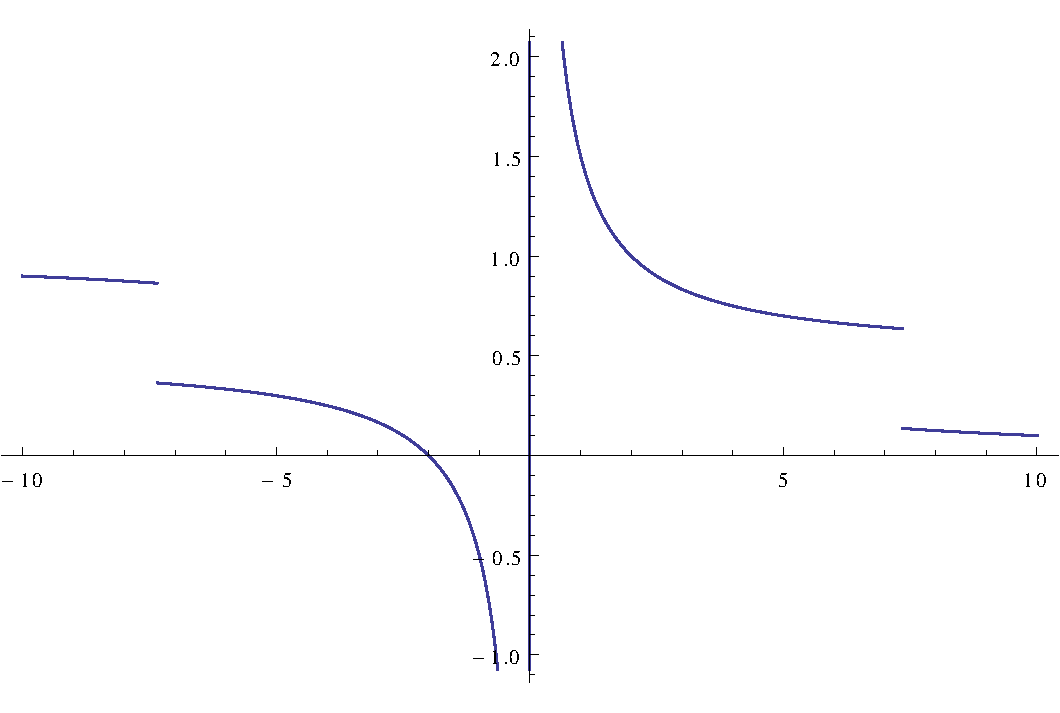
\includegraphics[width=\textwidth]{plot-stoerung.pdf}

Zu einer Zeit $t' > t$

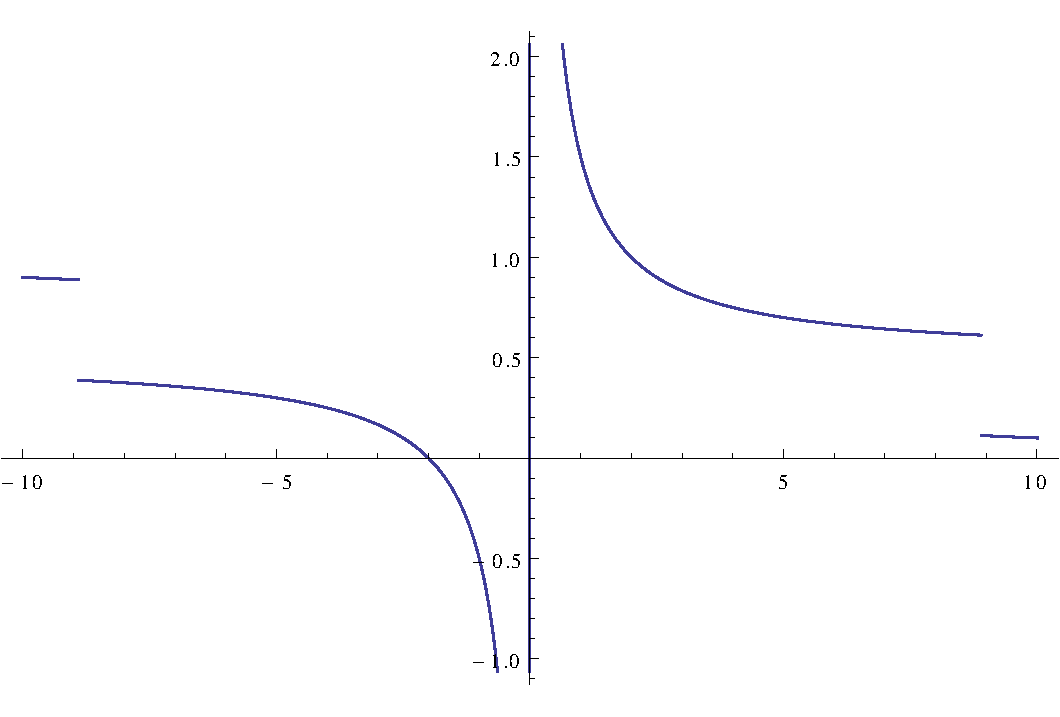
\includegraphics[width=\textwidth]{plot-stoerung2.pdf}


\end{document}
